\documentclass[times, utf8, diplomski]{fer}
\usepackage{booktabs}
\usepackage{listings}
\graphicspath{{./img/}}
\lstset{language=Python, tabsize=4, numbers=left, basicstyle=\small}

\begin{document}

% TODO: Navedite broj rada.
\thesisnumber{2451}

% TODO: Navedite naslov rada.
\title{Klasifikacija pokreta ljudskog tijela temeljena na podacima s inercijskih senzora}

% TODO: Navedite vaše ime i prezime.
\author{Ivan Trubić}

\maketitle

% Ispis stranice s napomenom o umetanju izvornika rada. Uklonite naredbu \izvornik ako želite izbaciti tu stranicu.
%\izvornik

% Dodavanje zahvale ili prazne stranice. Ako ne želite dodati zahvalu, naredbu ostavite radi prazne stranice.
\zahvala{}

\tableofcontents

\chapter{Uvod}
Karakteristike pokreta ljudskoga tijela vrlo su individualne te ovise o mnogo čimbenika kao što su genetika, odgoj te
fizička sprema. Ti pokreti su toliko jedinstveni da se mogu koristiti za identifikaciju osoba dok su s druge strane
toliko slični da čak i manje devijacije u tim pokretima također mogu ukazivati na neke zdravstvene probleme.
Ljudski pokreti mogu se klasificirati na razne načine koristeći računalni vid ili razne senzore postavljene na
ljudskome tijelu. Svaka od metoda ima svoju granu primjene kao: identifikacija osoba temeljenog na hodu koristeći
računalni vid na nadzornim kamerama \citep{surveillance}, pračenje pokreta igrača u interakciji sa igrama u virtualnoj stvarnosti \citep{VR},
korištenje inercijskih (IMU) senzora za precizno snimanje hoda u svhu otkrivanja bolesti i rehabilitacije te mnoge druge.

Klasifikacija pokreta vrlo je složen problem te kao takav nema dobro rješenje koristeći klasične algoritme. Razvojem moči računala
te metoda strojnoga učenja ovaj problem postaje rješiv. Za snimanje pokreta može se koristiti kamera ili senzori.
Koristeći kameru, na snimci se koriste metode računalnog vida te se traže karakteristike ljudskog tijela kako bi se na snimci
prepoznala osoba te koristeći te karakteristične točke analizira se hod. Također, kamera može snimati osobu sa posebno postavljenim
vizualnim oznakama po djelovima tijela te koristeći te vizualne oznake analizirati pokrete. Nedostatak kamera je taj što snimaju iz
jedne perspektive te zbog toga može doći do okluzije oznaka. Inercijski (IMU) senzori eliminiraju kamere te ne pate od problema okluzije.
Inercijski senzori su relativno jeftini i mali uređaji koji se postave na ključne djelove ljudskoga tijela te pružaju vrlo dobar uvid
u ljudske pokrete. Primjerice mogu se staviti na ruke te upravljati igrama i uređajima ali se mogu koristiti i u medicinske svrhe za
analizu hoda i diagnosticiranje zdravstvenih problema kao i za provođenje terapijskih vježbi bez nadzora stručnjaka.
Ovaj rad će se više fokusirati na medicinski aspekt klasifikacije pokreta, preciznije analizu hoda (\textit{eng.} gait) i terapiju koljena.



\chapter{Razrada}

\section{Bolesti koljena}

\section{Metode prikupljanja podataka}
Prikupljanje podataka o ljudskim pokretima može se odviti koristeći različite metode i tehnologije.
Svaka od tih tehnologija ima svoju granu primjene te možda neće biti adekvatna za primjenu u nekoj drugoj grani.

Prva razmatrana metoda prikupljanja informacija o pokretima je korištenje potisne ploče. Potisne ploče su elementi po kojima osoba
hoda te u sebi ima mjerač deformacija. Mjerač deformacija može biti ostvaren kao elastičan vodič vidljivim na slici \ref{defgag}. 

\begin{figure}[h!]
    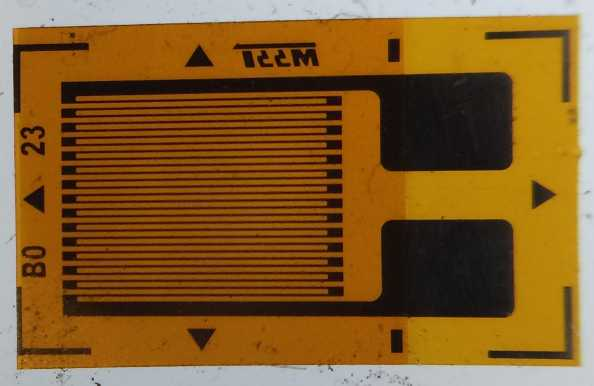
\includegraphics[width=\textwidth]{strain_gauge.jpg}
    \caption{Izgled mjerača deformacija (preuzeto sa \textit{wikipedia.com})}
    \label{defgag}
\end{figure}

Ovakav mjerač mjeri uzdužnu deformaciju na način da se elastični vodić prilikom deformacije izdulji odnosno suzbije
čime se zbog produljenja i sužavanja odnosno skračivanja i širenja vodiča mjenja ukupan otpor i time se deformacija može izmjeriti.
Ovisno o arhitekturi mjerača on mjeri deformaciju u nekome smjeru te kombinacijom više mjerača može se izmjeriti deformacija
u sve tri osi. Na taj način može se dobiti GRFV (eng. \textit{Ground Reaction Force Vector}) koji predstavlja, prema trećem Newtonovom zakonu,
sila reakcije i suprotna je utjecaju osobe koja djeluje na ploču. Osim ovakvih mjerača deformacija mogu se koristiti piezoelektrici
koji svojom deformacijom stvaraju razlike u potencijalima odnosno napon. Piezoelektrične potisne ploče su puno preciznije ali su
i znatno skuplje te ovisi o budžetu i o primjeni koja se tehnologija koristi. Ovakav pristup daje uvid isključivo u sile koje
djeluju na stopala i distribuciju težišta što je vrlo povoljno za analizu hoda ali i za ništa drugo. Potisne ploče vrlo su popularne
pri mjerenju performansa sportaša te mnogi profesionalne sportske ustanove i klubovi ulažu u vlastite ploče kako bi mogli nadzirati
svoje igrače. Ovakav pristup je korišten za prikupljanje jedne od najvećih baza podataka anotiranih za kliničku analizu \citep{pressurePlate}
opisanu u kasnijem poglavlju. Koristeći isti princip, kako bi se lakše mogle pratiti sile koje djeluju na stopala prilikom
raznih aktivnosti, moguće je napraviti uloške za cipele koje su također potisne ploče. Na ovakav način moguće je pratiti korake
ispitanika bez postavljanja više velikih potisnih ploča te ograničavanje ispitanika na samo tu manju površinu što je za potrebe
praćenja performansi sportaša u pojedinim sportovima idealno.

Jedna od metoda koja služi baš praćenju pocizicija donjih ekstremiteta je korištenje egzoskeleta. Egzoskelet je naprava koja se
postavi na vanjsku stranu ljudskoga tijela kako bi se njegovi djelovi kretali skupa sa djelovima tijela. Kako je svako tijelo
različitih dimenzija egzoskelet se mora moći namjestiti prema fizionomiji osobe na koju se postavlja kako bi zglobovi bili u
ravnini sa osovinama egzoskeleta. Za snimanje kretanja, na osovine egzoskeleta se postavljaju varijabilni otpori koji te osovine
pretvaraju u goniometar - uređaj koji mjeri kuteve. Svaki pokret zgloba može se zapisati kao promjena otpora u vremenu. Za to je
potrebno imati osovine na pordučju kukova, koljena i skočnih zglobova. Ovakav pristup puno vjernije snima pokrete tijela od potisnih
ploča jer se ne gleda samo sila na površinu koju vrši osoba već se precizno mjere kutevi njegovih ekstremiteta u vremenu. 


Problem korištenja egzoskeleta je taj što sam egzoskelet može značajno promjeniti način kretanja. Razlog tome je masa egzoskeleta
koja ovisi o materijalima i izvedbi te način pričvrščivanja za ljudsko tijelo. Također promjenjivi otpornici snimaju kuteve 
ekstremiteta u samo jednoj ravnini te ne snimaju niti konstrukcija dopušta moguću rotaciju ekstremiteta u drugim smjerovima.
Egzoskeleti mogu poslužiti za snimanje pokreta no njihova prava primjena nije u domeni prikupljanja podataka. Njihova primjena 
leži u robotskim egzoskeletima kakav je primjerice na slici \ref{exoskeleton}.

\begin{figure}
    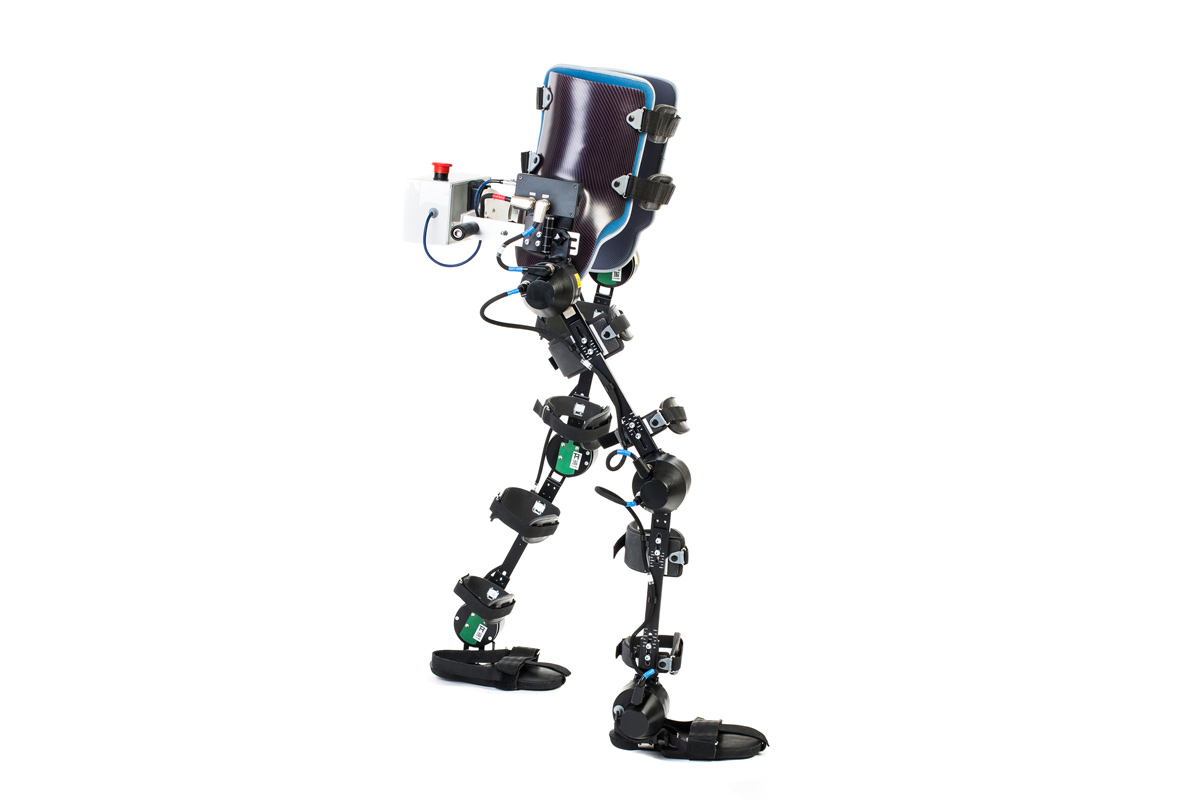
\includegraphics[width=\textwidth]{exoskeleton.jpg}
    \caption{Primjerak robotskog egzoskeleta Exo-H3 (preuzeto sa \textit{technaid.com})}
    \label{exoskeleton}
\end{figure}

Robotski egzoskeleti su naprave koje imaju isključivo senzore i snimaju pokrete već uz senzore imaju i aktuatore kao elektromotore.
Aktuatori glume ljudske pokrete i pomažu osobama sa poteškoćama. Jedna od glavnih primjena robotskih egzoskeleta je u fizikalnim
terapijama u kojima pacjenti zbog nekakve ozljede trebaju učiti ponovno hodati te pomažu nepokretnim osobama i osobama koje su
doživile moždani udar da postanu i ostanu mobilni. Potencijal ovakvih robotskih egzoskeleta je uvidila i vojna industrija te
je razvoj krenuo i u tom smjeru. U slučaju da osoba nije nepokretna moguće je iskoristiti senzore kako bi se pokreti snimali te
bi aktuatori istovremeno te pokrete izvodili \citep{exo}. Time se znatno rasterećuje ljudsko tijelo ali ovisno i o snazi aktuatora moguće je i
potencirati ljudsku snagu. Na taj bi način jedna osoba mogla podizati predmete znatno teže nego što bi ona to sama ikad mogla
napraviti i to bez ikakvog naprezanja jer bi cijela težina predmeta bila raspoređena na strukturi egzoskeleta a ne na ljudskom 
tijelu što značajno rasterećuje tijelo te se osoba vremenom ne umara. Ovakvu tehnologija se također razmatra za veliko unapređenje
radnih uvijeta u građevinskoj i logističkoj industriji jer bi se znatno umanjile nesreće uzrokovane padom predmeta zbog ljudske
istrošenosti i očuvala ljudska tijela jer nebi više dolazilo do pucanja mišića ili dobivanja bruha zbog prevelikog tereta na tijelu.

Kako sam egzoskelet znatno utječe na slobodno kretanje udova sljedeća razmatrana metoda prikupljanja podataka taj problem pokušava riješiti
bez naprava koje bi smetale snimanju slobodnog pokreta. Digitalne kamere snimaju kretanje osobe te kako nisu pričvršćene na osobu
na nikakav način ne utječu na njeno kretanje stoga je osoba u mogučnosti kretati se na najprirodniji mogući način. Ovisno o količini
okvira u sekundi kojom kamera snima osobu može se dobiti brzo uzorkovanje primjerice korištenjem vrlo brzih kamera sa i do
12600 okvira u sekundi ili korištenjem standardnih potrošačkih kamera do 100 okvira u sekundi. Idući od okvira do okvira osoba ručno
može označiti karakteristične točke na ljudskome tijelu te na taj način doći do podataka no takav postupak bi bio vrlo isrpan i
nepraktičan. Za automatizaciju tog postupka može se iskoristiti nekoliko različitih metoda. Prva razmatrana će biti korištenje
računalnog vida. Računalni vid je grana računalne znanosti koja se bavi načinom na koje računalo obrađuje digitalne slike i videe 
te razumjeva njihov sadržaj. Za rješavanje ovakve problematike se izdvajaju zavidna sredstva te je istraživanje došlo vrlo daleko.
Kina je jedna od zemalja koja ulaže puno sredstava u tehnologiju računalnog vida jer joj je u interesu koristiti tehnologiju za 
masovni nadzor građana. Nad snimkama s kamere se provodi analiza te je algoritam u mogučnosti prepoznati točnu osobu koja se na 
snimci nalazi u stvarnome vremenu. Na sličan način je moguče na snimci prepoznati ljudsko tijelo te označiti interesne točke kao zglobove ekstremiteta
te na taj način automatizirano prikupiti podatke o karakteristikama pokreta. Problem ovoga pristupa je ovisnost o osvjetljenju i o
dovoljno velikom kontrastu između osobe i pozadine kako bi algoritam pronašao željene točke. U slučaju da je kontrast suviše mali 
algoritam neće biti u mogučnosti prepoznati osobu ni interesne točke na snimci. Kada su laboratorijski uvijeti mogući koristi se
kombinacija pozadine i odjeće koja je vrlo kontrastna te koristeći jednostavnu obradu slike moguće je izdvojiti samu siluetu osobe
što znatno poboljšava rezultate algoritma i prepoznavanje pokreta.

Za povečanje preciznosti praćenja pokreta moguće je koristiti sljedeču razmatranu metodu a to je korištenje reflektirajućih markera
prilikom snimanja. Reflektirajući markeri su napravljeni po mogučnosti od retroreflektirajučih materijala (često poznatih pod nazivom
\textit{mačje oko}) koji iz bilokojeg kuta
mogu reflektirati izvor svjetlosti koji se nalazi pored objektiva kamere te postavljeni na ljudsko tijelo daju vrlo dobru oznaku
traženih točaka.
Prilikom obrade snimke te markere je vrlo lako izdvojiti jer su znatno svjetliji od svoje okoline te se na taj način može dobiti
vrlo precizna snimka pozicija tih točaka u prostoru. Kako bi ti markeri predstavljali dio tijela što preciznije potrebno ih je
postaviti na vrlo usku odjeću kako bi se kretali točno sa tijelom bez dodatnih smetnji koje bi kretanje tkanine proizvelo. Također
, kako se što većim kontrastom lakše detektiraju, ti markeri trebaju biti postavljeni na tamnu odječu, ovisno o primjeni crnu ili
sivu. Za još bolje rezultate mogu
se i iskoristiti i \textbf{aktivni} markeri koji su u suštini LED diode te emitiraju svjetlost što znači da ne ovisi o dodatnome
osvjetljenju za razliku od \textit{pasivnih} (reflektirajućih) markera koji samo reflektiraju već postojeće svjetlo. Ovakav pristup dopušta
postavljanje i pračenje proizvoljnog broja točaka na ljudskome tijelu. Jedini uvijet je da te točke budu dovoljno razmaknute jedne
od drugih kako bi kamera sa svoje udaljenosti mogla razlikovati svaku točku posebno. Kako je kamera uređaj koji snima dvodimenzionalnu
sliku iz perspektive u kojoj se nalazi postoji problem snimanja pokreta u tri dimenzije. Jedna kamera nije u mogučnosti uhvatiti
više dimenzija i adekvatna je za snimanje pokreta u dvije dimenzije slično kao i egzoskelet. Za dobivanje dubine moguće je ostvariti
stereoskopiju uz pomoć još jedne kamere, postavke koja je u svijetu poznata kao \textit{3D kamera}. Naime na taj je način moguće
dobiti informaciju o dubini no vidljivost markera još uvijek ovisi o perspektivi kamera te ovakva postavka je podložna problematici
okluzije. Okluzija se javlja u slučajevima kada marker iz pozicije kamere nije vidljiv jer se ili nalazi iza osobe ili neki drugi
predmet zaklanja pogled. U ovakvim slučajevima sustav za prepoznavanje pojedinih markera tretira isti marker kao dva različita
markera te se na taj segmentiran način podaci zapisuju. Kako bi se podaci povezali potrebno je manualnim putem tražiti takve markere
te na neki način interpolirati dio podatka koji zbog okluzije nedostaje kako bi se, ono što je sustav vidio kao dva različita
markera pretvorili opet u jedan kontinuirani. Zbog okluzije je moguće izgubiti velik broj korisnih podataka stoga je pozicija
kamera vrlo krucijalna. Kako bi se dobila kompletna snimka
pokreta u tri dimenzije potrebno je koristiti više kamera istovremeno. Te kamere moraju biti postavljene na način da u kadru postoji
preklapanje sa kadrom druge kamere kako bi se migracija markera iz kadra jedne u kadar druge kamere mogao pratiti i prepoznati
kao isti marker a ne kao dva različita. Za ovakvu postavu potrebno je imati minimalno tri kamere no više kamera predstavlja
manji rizik od javljanja okluzije.

Koristeći veliki broj kamera visoke rezolucije, mogučnosti snimanja velikog broja okvira u sekundi, postavljajući vrlo velik broj 
markera na tijelo te koristeći vrlo močna računala koja te snimke analiziraju te pretvaraju snimke u korisne podatke o pokretu
mogu se dobiti vrlo kvalitetni podaci. No toliko kvalitetni podaci imaju svoju cijenu koja je izvan budžeta večini ustanova te samo 
neke velike kompanije si ovakve sustave mogu priuštiti. Ova tehnologija je vrlo raširena u industriji računalnih igara
(eng. \textit{Gaming}) te filmskoj industriji za potrebe specijalnih efekata. Njihova uporaba i svrha tehnologije je vrlo slična.
U filmskoj industriji se češće koriste siva odjela sa markerima jer je osobama koje kasnije rade specijalne efekte u postprodukciji
vrlo bitno vidjeti izvor svjetla na filmskome setu te su markeri pasivni kako nebi nepoželjnim osvjetljenjem utjecali na svoju
okolinu u kadru. Također se u filmskoj industriji koristi manji broj kamera jer su kadrovi dvodimenzionalni i najčešće je samo
jedna kamera glavna dok nekoliko drugih kamera ima funkciju praćenja markera u prostoru. U industriji računalnih igara kadar nije
statičan već je potrebno vrlo precizno snimiti pokrete iz što više kuteva kako bi došlo do minimalne okluzije. Za to su primjereniji
aktivni markeri i crna odjela su preferabilna jer se dobije veći kontrast između tijela i markera a za razliku od filmske industrije
osvjetljenje nije bitno jer je mjesto radnje virtualno te se izvor svjetla postavlja programski. Također je poželjno vrlo precizno
snimiti pokrete iz svih kuteva zbog dinamične perspektive koja se u 3D igrama može mjenjati ovisno o poziciji i orjentaciji igrača,
stoga je potrebno imati što više kamera postavljnih oko površine na kojoj se osoba nalazi. Zahvaljujući tome glumac ili neka stručna 
osoba tipa majstor borilačkih vještina može svoju točku izvesti najbolje što može te se ti isti pokreti mogu primjeniti na likove
u igri te kao rezultat toga likovi u igrama imaju vjerodostojne, ljudske pokrete koje je nemoguće ostvariti umjetno. Također se u
obije industrije koristi specijalna kamera montirana na glavu osobe koja glumi te je usmjerena u lice na kojemu se također nalaze
markeri. Na ovaj način se maksimalno izbjegava okluzija markera te se snimaju pomaci pojedinog mišića lica tijekom glume kako 
bi se u procesu animacije dobili pravi ljudski izrazi lica. Ovakva postavka opreme je vidljiva na slici \ref{planet} na kojoj se
nalazi scena iz filma "Planet Majmuna: Revolucija" (eng. \textit{"Dawn of the Planet of the Apes}) (2014.) redatelja Matta Reevesa.

\begin{figure}[h!]
    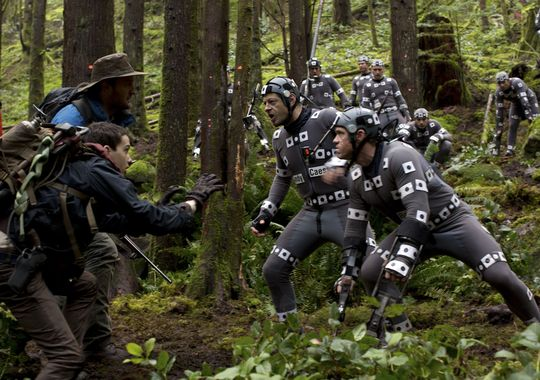
\includegraphics[width=\textwidth]{planet.jpg}
    \caption{Primjer opreme za pračenje pokrena u filmu (preuzeto sa \textit{aeromental.com})}
    \label{planet}
\end{figure}

Kako je već napomenuto ranije u poglavlju, ovakav sustav za praćenje pokreta ima veliki budžetni rang no jeftinije varijante su
vrlo neprecizne i podložne problemima okluzije dok su skuplje varijante suviše skupe ali zato i znatno preciznije. Također problem
je isto i sama infrastruktura i lokacija snimanja jer ovakva postava opreme je vrlo statična i zahtjeva studijske uvjete što si mnoge
ustanove nemogu priuštiti. Također veliki broj markera za potrebe klasifikacije pokreta nije potreban. Zbog svih ovih problema ovakvo 
rješenje se može iskoristiti no vrlo je skupo i operiranje ovakvom opremom je često vrlo zahtjevno te je iz tih razloga neadekvatno.

Zadnja razmatrana metoda je ona koja se u ovome radu koristi te ona uključuje korištene inercijskih (IMU) senzora. IMU senzori su
senzori koji se sastoje od akcelometra, žiroskopa i magnetometra. Korištenjem tih triju komponenti moguće je pratiti pokrete u
prostoru. Žiroskop daje informaciju o kutnoj brzini u određenoj osi, akcelometar daje informaciju o sili koja djeluje na njega
te magnetometar daje informaciju o magnetnom polju oko sebe koje uz odsudstvo bilokakvih metalnih predmeta i magneta daje informaciju
o orjentaciji senzora u zemljinom magnetnom polju odnosno služi kao svojevrsni kompas. Koristeći sve ove informacije moguće je
pozicionirati uređaj te pratiti pokrete uređaja. IMU senzori se nalaze u svakom pametnom telefonu kao senzor orjentacije kako bi se
prilagodila orjetacija ekrana, zapis o orjentaciji uslikanih fotografija ali i pojedini pametni telefoni kreativnije koriste IMU
senzore te se oni mogu koristiti za upravljanje nekakvih gestama primjerice trešnja pametnog telefona pali svjetlo kamere ili
okretanje telefona ekranom prema dole odbija dolazeći poziv i slično. Ovakvi senzori se također koriste za praćenje orjentacije
letjelica u zraku te za mjerenja i nadgledanja primjerice vibracija. Ono što se iz navedenih primjera može zaključiti oni su vrlo
malih dimenzija te kao takvi mogu biti postavljeni na bilokoje mjesto. Također zahtjevaju malo energije za svoj rad stoga se mogu
postaviti na neku udaljenu lokaciju gdje mogu snimati podatke. Cijena takvog senzora je vrlo pristupačna i minimalna cijena trenutno
je 3.33€ od kineskog nabavljaća preko stranice AliExpress.com što čini ovakve senzore vrlo povoljnima za nabaviti i koristiti u
većim količinama. Koristeći pseudoperiodičnost ljudskog pokreta proizvođači poput tvrtke Xiaomi su napravili uređaje za praćenje
tjelesne aktivnosti (eng. \textit{Fitness tracker}) u obliku sata koji koristeći IMU senzore mogu detektirati i brojati pojedini korak 
te koristeći BLE (eng. \textit{Bluetooth Low Energy}) telemetriju šalje na pametni telefon na kojemu aplikacija analizira signale
te može prepoznati različite aktivnosti primjerice sjedenje, hodanje, trčanje i slično koristeći samo jedan senzor.

Korištenjem više senzora postavljenih na udovima tijela moguće je puno preciznije snimati kretanja pri čemu osoba ima veliku slobodu,
veću negu u slučaju optičkog praćenja pokreta gdje se slobodno giba ispred kamera, veću nego u slučaju korištenja egzoskeleta u
kojemu sama naprava utječe na kretanje i snima podatke u samo jednoj ravnini te je moguće dobiti više podataka nego što to pružaju
potisne ploče. Osoba se može kretati bez prisustva druge osobe te se signali mogu snimati na memorijske kartice ili slati preko
interneta što čini ovakvu metodu prikupljanja podataka vrlo adekvatnim. U daljnjim poglavljima detaljnije se analizira
rad senzora te metode prikupljanja podataka i primjena tih podataka nad neuronskom mrežom kako bi se klasificirali pokreti donjih
ekstremiteta.

\section{Analiza IMU senzora}
IMU (eng. \textit{Inertial Measurement Unit}) je elektromehanički uređaj koji služi za mjerenje sila, kunih brzina te pozicije
uređaja koristeći skup senzora: akcelometar, žiroskop te magnetometar. Svaki od pojedinih senzora se sastoji od 3 manja senzora
koji svoj posao obavlja u odnosu na pojedinu os u prostoru. Oni u kombinaciji čine jednu jedinicu koja mjeri vrijednosti u sve 
3 prostorne dimenzije. Rane izvedbe ovakvoga senzora (poput one u Apollo 11 letjelici) su bile vrlo velikih dimenzija i nisu
u sebi imale magnetometar. Danas su se dimenzije IMU senzora znatno smanjile te je moguće izraditi sve potrebne komponente u
sklopu jednog čipa koristeći unaprijeđenja izrade sklopova u samom siliciju. Iako komponente jesu napravljene u siliciju one su
još uvijek elektromehaničke po prirodi što znači da se komponente slobodno gibaju unutar silicijske ploče na samome čipu
te su kao takve mikro-elektromehaničke (skračeno \textit{MEMS}). Danas su takvi uređaji nezamjenjivi u bilokakvim letjelicama a
pogotovo u bespilotnim letjelicama (eng. \textit{drone}) koji su u današnje vrijeme sve popularniji. Vrlo su bitni također u
navigacijskim uređajima jer u kombinaciji sa GPS uređajima daju dodatnu mogućnost pozicioniranja u slučajevima kada sam GPS signal
nije pristupačan kao što je to primjerice u tunelima te dodatno povećavaju preciznost pračenja kretanja. To je jedan od razloga
zašto je IMU senzor neizbježna komponenta pri izradi pametnih telefona. U rukama inženjera IMU senzori su dobili mnogo raznih 
kreativnih svrha te se mogu naći kao dio kontrolera u igraćim konzolama di služe kao dodatna metoda interakcije igrača sa igrom.
Prva promatrana komponenta bit će akcelometar.

\textbf{Akcelometar}

Akcelometar je senzor koji mjeri iznos sile u određenom smjeru. Jednostavan akcelometar se može konceptuirati kao masa ovješena na 
opruzi. Opruga se komprimira onoliko koliko je masa teška odnosno onoliko koliko je utjecaj gravitacije na tu masu. U slučaju
pojave nove sile u smjeru opruge ona se dodatno otpušta odnosno steže te je ukupan iznos sile na tijelo \textit{"pohranjen"}
unutar opruge odnosno istog je iznosa ali suprotne orjentacije. Kako bi se taj iznos mogao očitati u električnome obliku potrebno
je izvršiti pretvorbu a to se može ostvariti na dva načina, koristeći piezoelektrike te korištenje kapacitivnosti. Piezoelektrici
su materijali koji svoju deformaciju mogu pretvoriti u električni impuls te obratno, električni impuls mogu pretvoriti u mehaničku
deformaciju. Vrlo su korisni te njihova primjena varira od senzora koji vibracije akustičnih instrumenata pretvara u električne
signale kako bi se oni mogli snimiti i obraditi do okidača u đepnim upaljačima koji svojom deformacijom bacaju iskru potrebnu za
započimanje vatre. Od tog piezoelektričnog materijala se može napraviti opruga te bi kompresija i dekompresija opruge mogla davati
električni signal ekvivalentan iznosu sile na masu. Takva izvedba je vrlo skupa ali vrlo precizna za promatranje nekih pojava 
primjerice visokofrekventnih vibracija.

Druga mogučnost je korištenje kapacitivnosti kao mjeru kompresije i dekompresije opruge. Ako je masa ovješena na opruzi jedna ploča
kondenzatora, onda je površina na kojoj se sama opruga ovješena druga ploča kondenzatora. Ako su te dvije ploče pod naponom,
kompresija i dekompresija opruge približava i udaljava jednu ploču (masu) u odnosu na drugu ploču (površinu) te se kapacitet
povečava odnosno smanjuje što opisuje sljedeća jednadžba.

$$
C = \frac{\epsilon A}{d}
$$

Jedina promjenjiva varijabla je udaljenost $d$. Princip rada vidljiv je na slici \ref{accmtr}.


\begin{figure}[h!]
    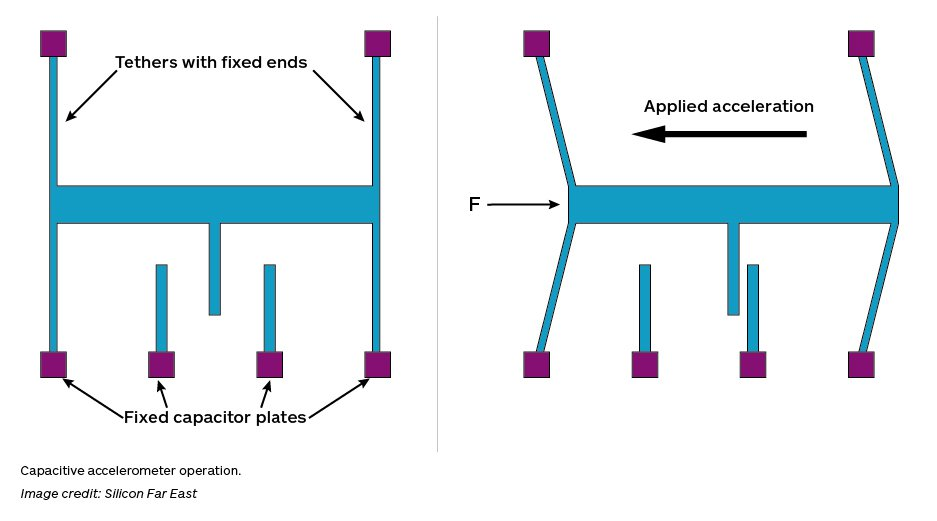
\includegraphics[width=\textwidth]{Accelerometers.jpg}
    \caption{Princip rada kapacitivnog akselometra (preuzeto sa \textit{insights.globalspec.com})}
    \label{accmtr}
\end{figure}

Kako bi se dimenzije akcelometra u potpunosti smanjile potrebno je razviti takav kapacitivni elektromehanički uređaj napravljen od
silicija koji bi bio u nekom od adekvatnih pakiranja za integrirane krugove. Također kako bi bili u mogučnosti promatrati silu u
prostoru potrebno je napraviti pojedini senzor za svaku od tri prostorne koordinate te kako bi one bile u što većoj mjeri usklađene
potrebno je sve ostvariti unutar jedne površine silicija kako bi bili skupa unutar integriranoga kruga u fiksnoj poziciji.

\textbf{Žiroskop}

Žiroskop je uređaj koji se sastoji od rotirajučeg diska koji se nalazi unutar kardanskog zgloba (eng. \textit{gimbal}). Rotirajuči
disk ima svoju kutnu količinu gibanja koja je promjenjiva jedino onda kada se na rotirajući disk djeluje silom, u protivnom
disk se rotira slobodno u ravnini u kojoj je zavrćen. Kardanski zglob je konstrukcija prstenja oko tog diska koji se oko diska
slobodno može rotirati u svim smjerovima bez da utječe na poziciju diska odnosno idejno ne djeluje silom na taj disk. Ovakav uređaj
je neznamjenjiv i jedan od najbitnijih komponenti svih letjelica jer uvijek letjelici daje referentnu točku iz koje se može
zaključiti točan položaj iste u zraku. Koristeći varijabilne otpore odnosno potenciometre postavljene na osovine kardanskog zgloba,
točna pozicija se može pretvoriti u električni signal koji se dalje može obrađivati i koristiti primjerice za
automatsku korekciju pozicije bilokakvog projektila ili letjelice što nudi mogučnost autopilota. Također, kako je brzina prva
derivacija puta u vremenu, tako je i kutna brzina derivacija promjene kuta u vremenu te se iz brzine promjene kuta može izračunati
i kutna brzina prilikom rotacije žiroskopa. Ovakva izvedba žiroskopa je
relativno velikih dimenzija te nikako nije primjerena za ugradnju u uređaje malih dimenzija kao što je to nekakav mobilni uređaj.
Za dizajn uređaja koji je dovoljno malih dimenzija potrebno je opet okrenuti se elektromehaničkim jedinicama implementiranim u poluvodiču.
Kod takve implementacije nije moguče imati rotirajuči disk i kardanski zglob što znaći da na ovakvoj skali nije moguće ostvariti 
pravi žiroskop koji bi konstantno pratio poziciju uređaja ali je moguće napraviti uređaj koji mjeri kutnu brzinu.
Takav uređaj se sastoji od vibrirajuće strukture, pojednostavljeno, dvije mase koje titraju u suprotnim smjerovima.
Prilikom rotacije, mase se više ne nalaze u inercijskom sustavu već u akceleriranome što znaći da na njih djeluju inercijalne sile.
Kada je sustav u rotaciji unutar njega djeluju razne sile kao što su centrifugalna, centripetalna i Coriolisova sila.
Coriolisova sila je inercijska sila koju tijela doživljavaju prilikom gibanja u rotiranom okviru promatranja. Sveprisutna je na 
planeti Zemlji te je vidljiva prilikom puštanja značajne količine vode u umivaoniku kao smjer vrtloženja vode i zaslužna za
uragane. Smjer djelovanja Coriolisove sile je okomit na smjer gibanja te na smjer rotacijskog vektora vidljivo na slici \ref{}.

%\begin{figure}[h!]
%    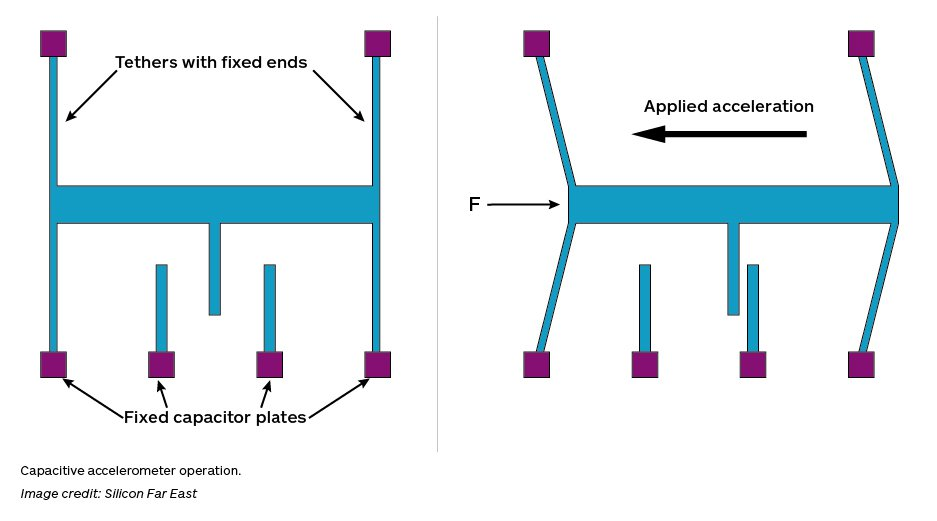
\includegraphics[width=\textwidth]{Accelerometers.jpg}
%    \caption{Princip rada kapacitivnog akselometra (preuzeto sa \textit{insights.globalspec.com})}
%    \label{accmtr}
%\end{figure}

\textbf{Magnetometar}

Magnetometar je senzor koji mjeri jačinu magnetnog polja koristeći pojave u elektromagnetizmu. Promjena magnetnog polja može
inducirati napon unutar vodića koji se nalazi u blizini no na taj se način može detektirati samo promjena. Za mjerenje magnetnog
polja koristi se Hallov efekt. Hallov efekt je fizikalna pojava koja javlja prilikom gibanja nabijene čestice kroz magnetno polje.
Električki nabijena čestica unutar magnetnog polja mjenja svoju putanju te počinje skretati i u slučaju gibanja po beskonačnoj
površini počinje svoje kružno gibanje pri čemu centripetalnu silu predstavlja Lorenzova sila. Pri ograničenoj površini nosioc
naboja putuje po vodiću prateći krivulju u smjeru u kojemu na njega djeluje Lorenzova sila te se na taj način istovrsni nosioci
nađu na istoj strani vodića te nisu nasumično raspršeni po njemu. Ta polarizacija predstavlja napon koji se može izmjeriti pri
čemu iznos tog napona ovisi o kutu između silnica magnetnoga polja i vodića te samom intenzitetu magnetnoga polja. Kako bi bi se 
nosioci naboja gibali unutar vodića potrebno je vodić spojiti na naponski izvor energije te kako bi oni imali prostora putovati na 
jednu od strana vodića on mora biti plosnat i veće površine. Primjer principa rada magnetometra vidljiv je na slici \ref{}.

%\begin{figure}[h!]
%    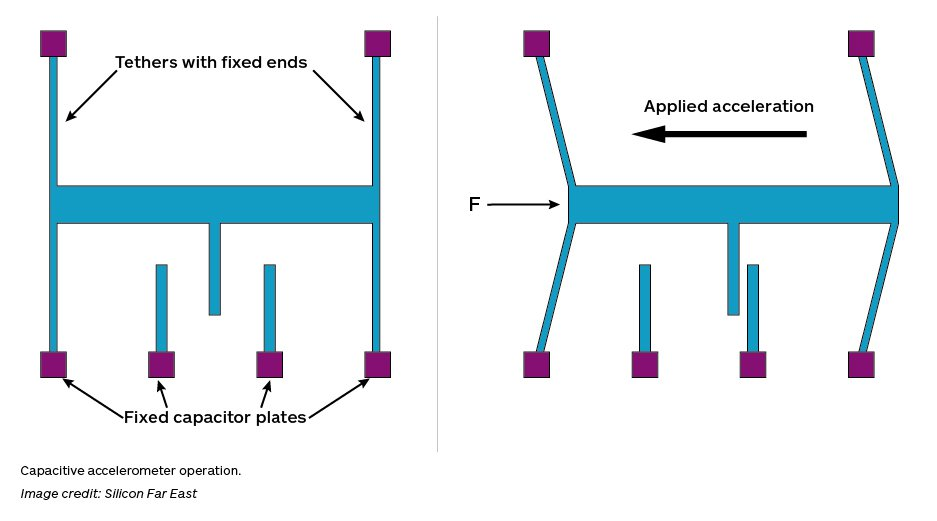
\includegraphics[width=\textwidth]{Accelerometers.jpg}
%    \caption{Princip rada kapacitivnog akselometra (preuzeto sa \textit{insights.globalspec.com})}
%    \label{accmtr}
%\end{figure}

Svaka od opisanih komponenata predstavlja samo dio pojedinog senzora i to dio koji mjeri pojave u samo jednom smjeru. Kako bi se
dobila kompletna slika potrebno je koristiti tri komponente, po jedna za svaki smjer u koordinatnom sustavu. Kako bi se to postiglo
potrebno je osmisliti arhitekturu poluvodičke pločice te paziti na preciznost i ispravno pozicioniranje svake komponente kako bi
ona mjerila točno svoj smjer u odnosu na druge. Ovakvi senzori dolaze često u pakiranju kao pojedini čipovi ili kao jedna cijela
IMU cjelina odnosno SiP (eng. \textit System in Package).

Ovakvih IMU sustava za razvoj uređaja na tržištu ima mnogo. Neki takvi su ICM-20948 tvrtke TDK i BMI serija IMU senzora tvrtke
Bosch koji su više industrijski orjentirani te postoje i oni orjentirani za hobiste i razvoj prototipova primjerice razvojne pločice
tvrtki \textit{Adafruit} i \textit{SparkFun}. Senzor ICM-20948 jedan je od najraširenijih IMU senzora u području znanosti i
industrije iz razloga što zahtjeva vrlo malo snage za pokretanje (2.5mW) \citep{ICM} što je vrlo proizvoljno 
za sustave napajane baterijom kao što su to mobilni telefoni ili nekakvi IoT (eng. \textit{Internet of Things}) uređaji.
Također nudi i digitalni procesor pokreta (eng. \textit{Digital Motion Processor - DMP}) koji služi tome da se algoritmi analize
pokreta mogu izvoditi na tom procesoru čime se rasterećuje glavni procesor ili mikrokontroler što dodatno štedi energiju. Dolazi u
QFN (eng. \textit{Quad Flat No-leads}) pakiranju te je u slučaju nabavke samo takvoga čipa potrebno je izraditi vlastitu tiskanu
pločicu što je poželjno u slučaju potrebe za nekim prilagođenim rješenjem no u slučaju izrade prototipa dodaje još jedan zahtjevan
proces u izradu što često nije poželjno. Neke kineske kompanije izrađuju već gotove tiskane pločice koje se mogu nabaviti, što je vrlo
poželjno za izradu prototipa. Druga vrsta takvih senzora su senzori za izradu jednostavnih prototipa i hobiste i primjeri takvih su
Adafruit L3GD20H i SparkFun Razor IMU. Adafruit IMU razvojno okruženje u sebi sadrži čip L3GD20H tvrtke ST te nudi priključke te
pretvarače napona kako bi se ova razvojna pločica mogla spojiti sa popularnim razvojnim okruženjima kao što je to Arduino ili
ESP32. Razor IMU sadrži čip MPU-5250 također tvrtke TDK koji je prethodnik već navedenog čipa ICM-20948 te u trenutku pisanja
ovoga rada je označen sa EOL (eng. \textit{End Of Life}) te proizvođač preporučuje korištenje trenutne ICM verzije čipa.
Popularna sučelja kojima se međusobno razvojne platforme i senzori povezuju su I2C i SPI. Bitna razlika između ICM-20948 i L3GD20H
je u logičkim naponskim razinama. ICM za komunikaciju koristi maksimalnih 1.95V \citep{ICM} što se bitno razlikuje od naponskih
razina razvojnih okruženja pri čemu Arduino koristi 5V TTL i ESP32 koristi 3.3V TTL. Za korištenje sa takvim okruženjima potrebno je
koristiti most za pretvorbu signala primjerice PCA9306 most za pretvorbu I2C signala korišten u \cite{mini_data_capture}.
Prednost ICM čipa u odnosu na ostale navedene je mogučnost napajanja naponom od 1.8V pri čemu zahtjeva 3.11mA struje.
U usporedbi sa L3GD20H kojemu je potrebno 3V te zahtjeva 5mA struje zahtjeva znatno manje snage što je primjerenije za rješenja
koja ovise o baterijskim napajanjima primjerice ugradbeni IoT sustavi ili mobilni telefoni. ICM može koristiti samo pojedine
komponente te svaka od komponenti može podržavati određenu brzinu uzorkovanja. Akselometar maksimalno može slati svoja mjerenja
frekvencijom od 4.5kHz, žiroskop 9kHz te magnetometar 100Hz. U dokumentaciji čipa L3GD20H nisu navedene točne frekvencije
uzorkovanja po komponenti, samo su navedene podržane frekvencije između 11.9Hz i 757.6Hz. Ove vrijednosti predlažu da je za
potrebu snimanja nekakvih visokofrekventnih vibracija bolji odabir ICM čip no za potrebe snimanja pokreta djelova tijela visoka
frekvencija nije bitan kriterij. Iz tog razloga valja razmotriti još jedan set IMU senzora a to je onaj koji se nalazi u pametnome
telefonu. Svaki pametni telefon u sebi ima jedan IMU senzor koji tom telefonu daje dodatne funkcionalnosti kao navigaciju, kompas,
rotaciju orjentacije ekrana i kao način upravljanja igrama. Mana ovoga pristupa je ta što sam model i specifikacija senzora
nisu javno dostupni podaci ne iz razloga tajnosti i intelektualnog vlasništva već proizvođači ne smatraju to bitnim informacijama.
Iz tog razloga nije moguće referencirati tehničku dokumentaciju i saznati neke ključne informacije u slučajevima kada je vrlo 
bitna preciznost i peformansa senzora. Prednost ovoga pristupa je ta što svi mobiteli podržavaju uzorkovanje frekvencijom od 
100Hz što je prema Nyquistovom teoremu ovoljno za snimanje periodičnih pokreta od gotovo 50Hz što je i više nego dovoljno.
Također ovakav pristup umanjuje e-otpad jer je jedan mobilni telefon već gotov sustav sa vlastitim napajanjem, načinom punjenja,
sučeljem za upravljanje (dodinik) te mogučnošću spremanja podataka odnosno slanja podataka preko bluetooth veze ili WiFi mreže.
Također pametni telefoni imaju u sebi vrlo močne procesore te bi se na njima mogla i izvoditi sama obrada podataka ukoliko za time
ima potrebe. Kako gotovo svaka osoba posjeduje minimalno jedan takav uređaj, skupljanje podataka u velikoj količini na taj način
postaje vrlo jednostavan i jeftin. Sličan pristup se koristi u \cite{android}, radu koji koristi samo jedan IMU senzor
postavljen na polovici potkoljenične kosti te uzorkuje signal frekvencijom od 102.4Hz te putem bluetooth veze šalje podatke na 
pametni telefon na kojemu se sami podaci obrađuju te je preciznost prepoznavanja pokreta vrlo visoka.

\section{Analiza dostupnih baza podataka}
Mnogo je znanstvenih radova napisano na temu ljudskih pokreta i analizu istih. Kako bi se ljudski pokreti analizirali potrebno ih 
je na neki način snimiti a to se može ostvariti jednom od metoda analiziranih u pijašnjem poglavlju. Kako bi znanost mogla
napredovati te kako bi se drugi ljudi mogli uvjeriti u rezultate rada, mnogi autori svoje podatke stavljaju javno dostupnima.
Ovo će se poglavlje baviti analizom već dostupnih baza podataka, metodom prikupljanja tih podataka te njihovom svrhom.
Većina dostupnih podataka su prikupljeni podaci o hodu (eng. \textit{gait}). Razlikuju se u broju sudionika, metodi prikupljanja
podataka, i svrsi prikupljanja tih podataka.

Prva razmatrana baza podataka je \texttt{whuGAIT} autora \cite{zou2020gait}. U svome radu autori razmatraju mogučnost biometrijske
identifikacije i autentifikacije osoba koristeći specifične karakteristike hoda. Skup podataka sastoji se od podataka prikupljenih
sa pametnog telefona koji se nalazio u džepu osobe koja je bila snimana pri čemu su se snimali tri osi akselometra i tri osi
žiroskopa frekvencijom uzorkovanja od 50Hz. U prikupljanju podataka je sudjelovalo 118 različitih osoba. Skup podataka je podjeljen
u 8 podskupova od kojih su podskupovi 1-4 namjenjeni za identifikaciju osobe, 5 i 6 za autentifikaciju i skupovi 7 i 8 za
razdvajanje podataka između onih u kojima se vrši hodanje i onih u kojima se ne hoda kako bi se korištenjem neuronske mreže
razdvojio kontinuirani tok podataka. U svim podskupovima su podaci zapisani u tekstualnu datoteku kao CSV vrijednosti. Svaka
tekstualna datoteka predstavlja jednu os akselometra odnosno žiroskopa te svaka linija unutar datoteke je uzorak hoda neke osobe.
U posebnoj datoteci se nalaze brojevi koji predstavljaju pojedinu osobu kojoj snimka hoda pripada. Svrha ovih podataka je treniranje
neuronske mreže koja rješava problem n-klasne klasifikacije odnosno pokušava prepoznati i identificirati odnosno autentificirati
osobu bazirano isključivo na njezinom hodu. Koristeći ove podatke \cite{zou2020gait} su dobili preciznost od 93\% u identifikaciji 
i autentifikaciji no ovi podaci nisu iskoristivi za klasifikaciju pojedinog pokreta jer nije anotirana za pojedine pokrete te se 
ne može iskoristiti za treniranje takve mreže no pokazuju da je moguće snimiti vrlo precizne karakteristike pokreta koristeći samo 
jedan pametni telefon.

Sljedeća razmatrana baza podataka je ona koju su snimili \cite{uneven}. Njihov cilj je bio napraviti bazu koja sadrži podatke o
načinu hoda po raznim površinama kako bi uvidili performanse hoda. Prilikom snimanja sudjelovalo je 30 osoba (15 ženskih i
15 muških). Svaka osoba je na sebi imala po 6 IMU senzora: lijeva i desna potkoljenica, lijeva i desna nadkoljenica, donji dio leđa
oko L1 kralješka i desno zapešće. Svaka osoba je hodala ravno bez promjene smjera 6 puta po ravnoj asfaltiranoj površini, uzbrdici
odnosno nizbrdici, stepenicama u oba smjera, travnata površina, neravna kamena cigla i šljunak. Podaci svakoga od 6 senzora su
pohranjeni u svojoj CSV datoteci označenoj šifrom iz koje je vidljivo na kojoj se lokaciji nalazio senzor te po kojoj površini
osoba hoda. Podaci svake pojedine osobe se nalazi unutar vlastitog direktorija. Svaki hod unutar direktorija dolazi i sa binarnom
datotekom koja predstavlja te podatke. Uz sve te podatke \cite{uneven} su također obradili i uveli u \textit{Matlab} datoteku pod 
imenom \texttt{data.mat}. Ovakva baza podataka nudi razne mogučnosti poput klasificiranja površine po kojoj osoba hoda ili samo 
detekcija hoda opčenito neovisno o površini. Autori su ponudili svoju bazu podataka sa svrhom da unaprijede već postojeće baze
ljudskoga hoda koje su zbog tehničkih ograničenja snimane isključivo u laboratorijskim uvijetima te kao takve nisu bile primjerene
za primjere iz stvarnoga svijeta. Razvojem IMU tehnologije i bežićne komunikacije \cite{uneven} odlučili su napraviti set podataka
snimajući hod u stvarnome svijetu. Ova baza podataka također nije primjerena za potrebe ovoga rada jer su anotirani samo tereni
po kojima ispitanici hodaju te se ne klasificira pokret.

Bazu podataka pod imenom \texttt{HuGaDB} su ostvarili \cite{HuGaDB}. Prilikom provedbe radnji snimljeno je 18 različitih sudionika
koji su imali 6 IMU senzora na sebi te 2 EMG senzora. IMU senzori su postavljeni na nadkoljenice, podkoljenice te stopala sudionika
pri čemu su snimali radnje: hodanje, trčanje hodanje uz stepenice, hodanje niz stepenice, samo sjedenje, sjedenje iz stajačeg položaja,
ustajanje iz sjedećeg položaja, stajanje, voženje bicikla, dizanje unutar dizala, spuštanje unutar dizala i sjedenje
u automobilu kao putnik. Sve radnje su u potpunosti segmentirane što znaći da su ispravno anotirane te spremne za treniranje
neuronske mreže. Podaci su pohranjeni u tekstualne datoteke u kojima svaki stupac predstavlja vrijednosti pojedinog segmenta
svakog senzora pri čemu je pozicija senzora označena sa oznakom strane na kojoj se nalazi R i L te pozicijom na nozi F, S i T
(eng. \textit{Foot, Shin i Thigh} redom). Uz poziciju senzora oznaka \textit{acc} i \textit{gyro} označava pojedinu komponentu
IMU senzora te oznake \textit{x, y i z} predstavljaju pojedinu os. Tako jedan segment s oznakom \texttt{acc\_rs\_x} označava
podatke akselometra na desnoj potkoljenici u x osi. Svaka tekstualna datoteka se sastoji od identifikatora sudionika,
rednog broja ponavljanja, aktivnosti, verzije i prefiksa koji označava datoteku sa podacima. Tako primjerice datoteka sa imenom
\texttt{HGD\_v1\_walking\_17\_02.txt} označava podatke prve verzije baze podataka u kojoj osoba pod rednim brojem 17 hoda po
drugi put. Autori \cite{HuGaDB} na svojoj \textit{github} stranici nude već gotove skripte koje služe učitavanju podataka u
matlab i python programe te skriptu koja tekstualne datoteke pretvara u \textit{SQLite}. bazu podataka.
Ova baza podataka se ne bavi pojedinim djelom tijela no uzimajući samo podskup 
senzora bilo bi moguće ostvariti prepoznavanje akcije poput vožnje bicikla, hodanja i slično što je puno bliže klasifikaciji pokreta
kakva se razmatra u ovome radu. Problematika ove baze podataka je navedena u uputstvima te nalaže da su zbog greške u žiroskopu
neke vrijednosti krive jer je snimak pojačan 10 puta što je dovelo do \textit{klipinga} te je takav signal gotovo neiskoristiv.
Svaki takav slučaj je dokumentiran u tablici te se po potrebi ti podaci mogu izbjeći.

Poslijednja razmatrana baza podataka je jedna od najvećih baza podataka hoda sa kliničkim anotacijama koju su snimili \cite{pressurePlate}.
Podaci su prikupljani u Austrijskom rehabilitacijskom centru od 2007. do 2018. godine. U prikupljanju je sudjelovalo 2085 pacjenata.
Svaki je pacjent trebao bez ikakvih pomagala prehodati 10 metara preko potisnih ploča (eng. \textit{Pressure plate}) koje su snimale
GRF (eng. \textit{Ground Reaction Force}) odnosno silu pritiska stopala. Svaki pacjent je svoj hod ponovio 10 puta te je ponavljao
hod na tjednoj bazi. Snimke su anotirane prema dijagnozi te prema razini rehabilitacije kako bi se mogle usporediti i sa drugim
pacjentima te kako bi imali uvid u proces rehabilitacije. Problematika ove baze podataka je u tome što se za snimanje pokreta ne
koriste inercijski senzori već se koristi set potisnih ploča koje snimaju samo težinu kojom pacjenti djeluju na njih te takva baza 
podataka nije primjerena za analizu pojedinih pokreta već samo hoda.



\section{Stvaranje vlastite baze podataka}
Za stvaranje vlastite baze podataka potrebno je definirati svrhu i ciljeve te baze a zatim odrediti metodu prikupljanja podataka. U ovome će radu
fokus biti primarno na stvaranje baze podataka korisne za analizu pokreta koja bi se mogla upotrijebiti u svrhe fizikalne terapije koljena.
Za snimanje općenitih pokreta može se iskoristiti mnogo senzora postavljenih po cijelome tijelu ali za potrebe snimanja jednoga zgloba potrebno je 
koristiti dva senzora, po jedan sa svake strane uda kojeg zglob povezuje. U konkretnom primjeru koljena to su nadkoljenica i potkoljenica.

Ovisno o razini preciznosti, cjeni i dostupnosti potrebno je odabrati i same senzore za prikupljanje podataka. Redovito se sustavi senzora
za istraživačke svrhe rade baš za tu namjenu te postoji mnogo sustava otvorenog koda i otvorenih komponenti koji se mogu iskoristiti. Razni
proizvođači nude i svoja već gotova komercijalna rješenja za koje garantiraju rad i pružaju podršku ali takvi sustavi ponekad nisu adekvatni za
istraživačke svrhe zbog svoje zatvorenosti i potencijalnog manjka interoperabilnosti sa drugim uređajima i programima. U ovome radu, zbog jednostavnosti,
koristiti će se pametni telefon.

Tipičan životni vijek jednog pametnog telefona u prosjeku je dvije godine nakon čega korisnici redovito kupuju nove modele jer stariji postaju neadekvatni
po pitanju trajanja baterije, količine memorije, performansama komponenti i slično. Svaki takav stariji model telefona vrlo često stoji nekorišten iako je još uvijek
funkcionalan. Gotovo svaki pametni telefon u sebi sadrži IMU senzor te u sebi već ima povezivosti poput \textit{WiFi i Bluetooth}. Uzimajući u obzir
također da pametni telefoni imaju i ugrađenu bateriju koja može još uvijek biti dovoljno dugotrajna, ekran osjetljiv na dodir kao metodu interakcije i to 
sve ukomponirano u uređaj koji svojim dimenzijama stane u džep dolazimo do zaključka da su pametni telefoni i više nego adekvatni za prikupljanje podataka.
Također, vrlo je realna pretpostavka da svaka osoba ima pristup minimalno jednome, vjerojatno i dva pametna telefona što čini prikupljanje velike količine
podataka od većeg broja sudionika znatno jednostavnijim. Koristeći držaće pametnog telefona za trčanje ili marama, uređaji se mogu postaviti osobi na bilo koji
dio tijela vrlo jednostavno i svaka bi osoba iz svoga doma mogla pridonjeti stvaranju baze podataka.

Aplikacija koja očitava vrijednosti može biti napravljena posebno, no na tržištu postoje gotove aplikacije, redovito otvorenoga koda, koje se već time bave.
Bitno je pronaći odgovarajuću aplikaciju no u slučaju da takva ne postoji potrebno je izraditi svoju. Mnoge aplikacije u trgovini ne nude selekciju samo određenih senzora
već snimaju sve senzore kojima pametni telefon raspolaže, te u većini slučajeva nude formatiranu pohranu podataka isključivo u memoriju uređaja što je vrlo neadekvatno ako bi se uređaji
koristili primjerice za obradu informacija u stvarnome vremenu ili za centralizirano prikupljanje podataka primjerice na računalo. Neke od takvih aplikacija su
\textit{Sensor Data} i \textit{phyphox} koje se koriste u edukaciji te su u doba COVID pandemije nezamjenjivi alati za vršenje fizikalnih eksperimenata kao dio
školske zadaće. Nedostatak ovih aplikacija je taj što sve podatke snimaju na lokalnoj memoriji uređaja te nisu primjerene za obradu podataka u stvarnome vremenu.
Aplikacija \textit{Sensorstream IMU+GPS} ne nudi grafičke prikaze podataka već u svojoj vrlo bazičnoj funkcionalnosti nudi odabir senzora uz prikaz trenutnih
vrijednosti istih te odabir akcije koju želimo napraviti sa tim podacima. Ponuđene su funkcije spremanja vrijednosti u CSV (\textit{Comma separated value}) formatu,
slanje podataka koristeći UDP protokol te kombinaciju oboje. Za slanje podataka korištenjem UDP protokola potrebno je navesti određenu IP adresu uređaja te \textit{port} na
kojemu uređaj očekuje promet. Također nudi 4 frekvencije uzorkovanja označene sa \textit{slow, medium, fast i fastest}. Te frekvencije uzorkovanja nisu dobro dokumentirane
te nigdje nije navedeno koliko one iznose zapravo. Za mjerenje tih frekvencija može se iskoristiti alat \textit{wireshark}. Wireshark je alat otvorenoga koda koji
služi za analizu mrežnoga prometa. Vrlo raširen i nezamjenjiv alat za svaku granu računarstva koja se bavi mrežnim prometom. Nudi razne opcije od kojih je jedna 
od močnijih ugrađeni filter koji vrlo precizno može naći određeni paket unutar snimke mrežnog prometa. Koristeći tu mogučnost promet se može snimiti na računalu
te kasnije filtrirati samo one pakete koje mobilni uređaj šalje. Gledajući vremenske indekse prvoga i posljednjega paketa dobivamo ukupno trajanje
snimanja te znajući točan broj paketa može se izračunati približna frekvencija uzorkovanja te su one prikazane u tablici \ref{frekvencije}.

\begin{table} [h!]
 \centering
    \begin{tabular}{|c|c|c|c|}
        \hline
        Uzorkovanje & Trajanje (s) & Broj poruka & Frekvencija \\
        \hline
        Slow & 12.21 & 61 & 5 \\
        Medium & 3.98 & 61 & 15 \\
        Fast & 6.85 & 344 & 50 \\
        Fastest & 2.14 & 299 & 124\\
        \hline
    \end{tabular}
    \caption{Izmjerene frekvencije uzorkovanja}
    \label{frekvencije}
\end{table}

Također koristeći wireshark alat može se jedan paket analizirati i vidjeti format podataka koju uređaj šalje. Podaci su u CSV formatu u kojima se šalje vremenski indeks,
identifikacijski brojevi senzora te same vrijednosti senzora kako se vidi u slici \ref{datagram}. Svi podaci prikazuju vrijednosti redom $x$, $y$, i $z$ osi.

\begin{figure}[h]
    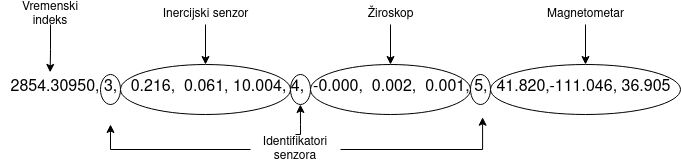
\includegraphics[width=\textwidth]{datagram.png}
    \caption{Primjerak primljenih podataka}
    \label{datagram}
\end{figure}

Kako bi se ti podaci primili i pohranili na adekvatan način potrebno je napraviti program klijent koji osluškuje na određenim portovima. Implementacija tog programa 
u ovome radu biti će napravljena koristeći skriptni jezik python. 

Python je vrlo popularan jezik mnogih mogučnosti koji je vrlo jednostavan za naučiti i koristiti te zbog svoje popularnosti raspolaže mnogim bibliotekama.
Neke od tih vrlo korisnih biblioteka koje će biti korištene u ovome radu su \textit{numpy}, \textit{matplotlib} te \textit{socket}. Python se kao skriptni jezik
izvodi liniju po liniju te se svaka linija iterpretira tek kad ona dođe na red za izvršavanje što ukida proces prevođenja programa u strojni kod kao što je to primjerice
potrebno kod programskog jezika \textit{C}. Iz tog razloga je vrijeme izvršavanja takvoga koda znatno dulje što znatno utječe na performanse programa. Kako bi se
izvođenje kompliciranijih matematičkih operacija znatno ubrzalo te kako bi se ponudio veći opseg već gotovih funkcija napravljena je biblioteka \textit{numpy}.
Numpy je biblioteka koja nudi gotovo sve potrebne funkcije za izradu programa koji se koriste u znanosti. Implementira višedimenzionalne matrice te sve funkcije
za operaciju nad njima uključujući promjenu oblika matrice te sve matrične operacije. Također nudi i funkcije za Fourierovu transformaciju, statističku obradu,
generatore nasumičnih brojeva i slično. Numpy implementacija matrica je znatno bliža onakvim matricama kao što su u programskome jeziku C te su kao takve memorijski
znatno manje zahtjevne od originalnih matrica koje nudi python. Također kako bi operacije nad matricama bile brze operacije su implementirane u programskome jeziku C te
prevedene unaprijed tako da biblioteka nudi vrlo jednostavnu sintaksu uz jako veliku brzinu izvođenja te manju veličinu datoteke pri pohrani podataka.
Biblioteka \textit{socket} nudi funkcije za umreživanje koje su potrebne kako bi se podaci uspješno primili sa mobilnih uređaja je \textit{matplotlib} koji je potreban
za vizualizaciju podataka u obliku grafova.

\begin{lstlisting}[caption=Ostvarivanje veze na strani klijenta, label=socket]
def init_client(srv_port):
    client_socket = socket.socket(family=socket.AF_INET,\\
                                    type=socket.SOCK_DGRAM)
    client_socket.bind((self_ip, srv_port))
    return client_socket

client = []

client.append(init_client(port))
print("UDP client up") 
\end{lstlisting}

U kodu \ref{socket} je vidljiv način na koji se koristi biblioteka \textit{socket}. Svaki mobilni uređaj predstavlja instanca klase \textit{socket} koja se sprema
u listu klijenata \texttt{client} što omogučuje povezivanje proizvoljnog broja mobilnih senzora pri čemu svaki senzor treba imati svoj poseban port. Port na računalu
bi trebao biti slobodan odnosno niti jedna druga aplikacija ne bi smjela koristiti taj port za svoj promet. Dobra praksa nalaže da se za osobne potrebe koriste portovi
brojeva većih od 1024 kako bi se izbjegli moguči zauzeti portovi nekakvih standardnih protokola kao što su \textit{https} i slični. U ovome slučaju mobilni uređaj
s indeksom 0 koristi port broja 5555 te svaki sljedeći zauzima port $5555 + i$ pri čemu je $i$ indeks uređaja. Točan broj je potrebno unjeti ručno na svaki uređaj
koji šalje podatke. Stvaranje instance \textit{socket} odvija se u liniji 2 i 3 pri čemu se u argumentu treba navesti tip veze. Za familiju veze se navodi
\texttt{AF\_INET} što predstavlja IP protokol te pod tip se navodi \texttt{SCOK\_DGRAM} što označava korištenje UDP protokola. UDP (eng. \textit{User Datagram Protocol})
je jedan od osnovnih transportnih protokola koji podatke prenosi po principu \textit{best effort}, pretpostavlja se da su datagrami došli do odredišta u ispravnome redosljedu
te se ne potvrđuje primitak datagrama. Ovakav protokol ne garantira cjelovitost podataka no nudi manje zagušenje prometa zbog nedostatka potvrđivanja svakog primljenog
datagrama i retransmisije u slučaju gubitka te se iz tog razloga koristi za prijenos videa ili VoIP (eng. \textit{Voice over IP}) pozive. U liniji 4 se instanca razreda
\textit{socket} povezuje s odgovarajučim portom na odgovarajučem mrežnom uređaju koji je predstavljen vlastitom IP adresom \texttt{self\_ip}. Na kraju funkcija
\texttt{init\_client} vraća instancu kako bi bila spremljena u klijentsku listu.

\begin{lstlisting}[caption=Primanje podataka, label=primanje]
while(True):
    sample = []
    for phone in client:
        bytes_adress_pair = phone.recvfrom(buffer)
        data = []
        message = bytes_adress_pair[0].decode().split(",")
        for i in message:
            data.append(i.strip())

        # filteri podataka
        if "4" not in data:
            continue

        for i in data_filter:
            data.pop(i)
        
        if len(data) != 0:
            sample.append(data[:6])
            
    if len(sample) != 0:
        signal.append(sample)
    else:
        continue
\end{lstlisting}

U odsječku koda \ref{primanje} prima se datagram svakog mobilnog uređaja. Svaki datagram se uzima iz međuspremnika koji je veličine 1024 bajta. Svaki datagram se sastoji
od samih podataka (u 6. liniji koda pod indeksom 0) te IP adrese pošiljatelja koja u ovoj implementaciji nije potrebna te se može izostaviti. Nad podacima se vrše obrade
poput uklanjanja bjelina (linija 8.) te rastavljanje podataka iz jednog monolitnog zapisa podataka u više posebnih podataka pomoću \texttt{split} funkcije uzimajući
zarez kao graničnik. Zatim te podatke valja filtrirati pri čemu se uklanja \textit{vremenski indeks}, identifikatori senzora te podaci magnetometra
vidljivi na slici \ref{datagram}. Eksperimentalno se pokazalo da se pri prvih nekoliko mjerenja od početka slanja podataka sa mobilnih uređaja izostavljaju vrijednosti
žiroskopa te se gledajući prisutnost tih vrijednosti dodatno vrši čekanje na spremnost svih senzora u mobilnome uređaju. U ovome kodu to se vrši uvjetovanjem u liniji 11.
Struktura podataka je prikazana u slici \ref{struktura}.

\begin{figure}[h]
    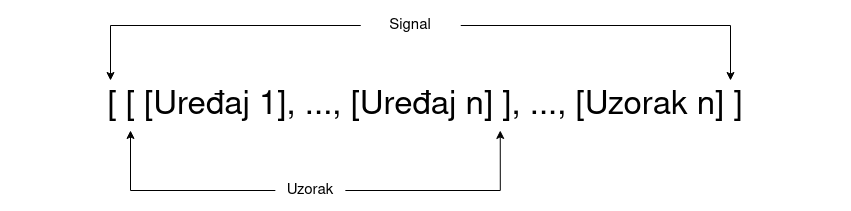
\includegraphics[width=\textwidth]{OrganizacijaPOdataka.png}
    \caption{Struktura podataka}
    \label{struktura}
\end{figure}

Uzorak jednoga uređaja je lista vrijednosti njegovih senzora. Jedan uzorak je lista uzoraka \textbf{svih} uređaja. Signal je samo lista uzoraka. Na ovaj se način akcija 
može snimiti i koristeći biblioteku \textit{numpy} pohraniti na računalo za daljnju obradu.

Kako bi se prikupili odgovarajući podaci za treniranje i uporabu neuronske mreže potrebno je iz toka podataka izdvojiti pojedina ponavljanja vježbi kako bi samo ti bitni
segmenti ili bili prikupljeni za treniranje neuronske mreže ili kako bi se pojedini segment predao neuronskoj mreži na klasifikaciju. 
Mnogi radovi primjerice \cite{android}, \cite{exo} i \cite{LowerLimb} spominju pronalazak karakterističnih točaka unutar signala
kao jednu od glavnih faza predobrade signala. Ovisno o željenom rezultatu moguće je promatrati statičke osobine signala
kao što su to prosjek, standardna deviacija, variancija i slično te dinamičke kao što su to energija, prosjek energije, odnos
harmonika, energetska entropija i slično \citep{android}. Također je moguće napraviti posebne klasifikatore koji su u suštini
neuronske mreže trenirane posebno za detekciju pojedinih osobina signala kao što su to napravili \cite{exo}. 
Najjednostavniji pristup tome je promatranje samo jedne osi određenoga senzora u nekome vremenskom periodu kao što su to napravili
\cite{LowerLimb}. Promatranjem samo jedne osi jednoga senzora fokus može biti na pseudoperiodičnosti tog signala te se detekcija
periodičnosti i segmentacija može odviti pomoću detekcije rubnih vrijednosti. Izvođenjem jednostavnije vježbe poput ispruživanja
potkoljenice (eng. \textit{leg extension}) s obzirom na poziciju mobilnog uređaja koji se nalazi ekranom okrenutim od potkoljenice uspravno na
potkoljenici može se sav fokus staviti na vrijednosti žiroskopa u $x$ osi. Snimajući te iscrtavajući odgovarajuče vrijednosti
na grafu vrlo je jasno vidljiv period te same karakteristike funkcije (slika \ref{period}). Dok se vježba ne izvodi signal je
vrlo miran i iznosi približno 0. U trenutku početka pružanja potkoljenice zbog smjera rotacije mobilnog uređaja kutna brzina iznosi
otprilike $-2.5 rad/s$. Zatim se potkoljenica u stanju potpune ispruženosti smiri te kutna brzina iznosi 0. Pri spuštanju kutna
brzina raste te također iznosi približno $2.5 rad/s$, ali u ovom slučaju u pozitivnom smjeru. Uzeći ove vrijednosti može se ostvariti
konačan automat koji prati vrijednosti signala te mjenja stanja u odnosu na iste pri čemu se pamti početak perioda. Ako se automat nađe u
prihvatljivom stanju onda to predstavlja kraj periode te je poznat cijeli segment signala koji predstavlja jedno ponavljanje.

\begin{figure}
    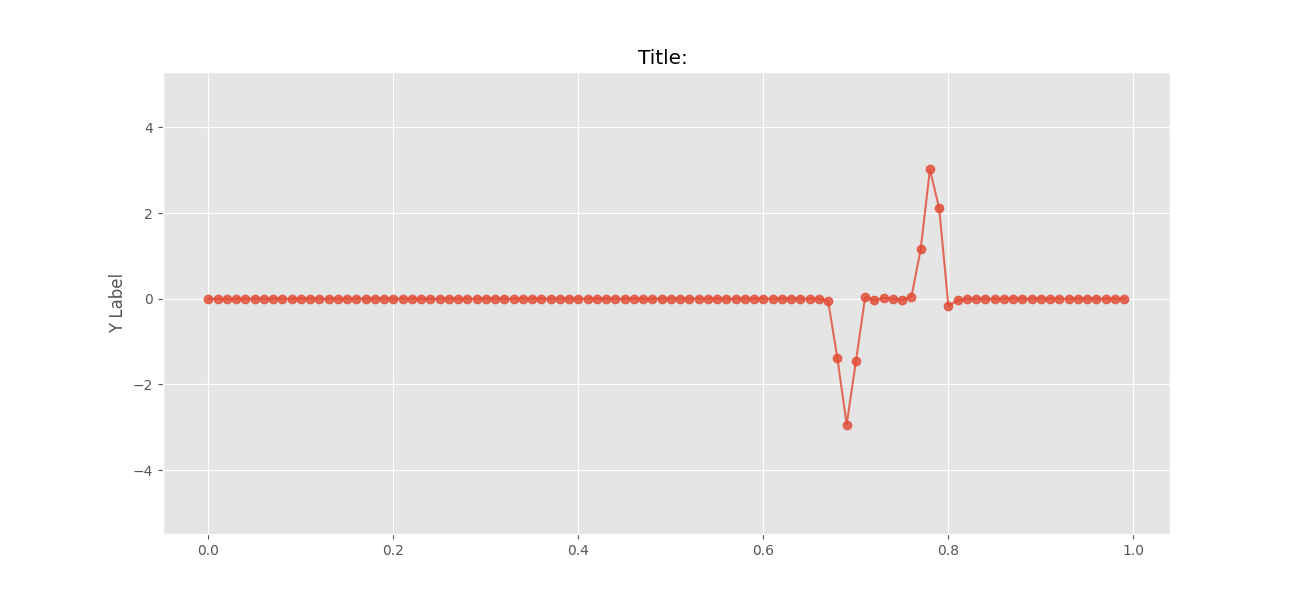
\includegraphics[width=\textwidth]{period.png}
    \caption{Primjer jednog ponavljanja vježbe, x - vrijeme, y - kutna brzina}
    \label{period}
\end{figure}

\section{Implementacija metode strojnoga učenja}

\section{Rezultati}

\chapter{Zaključak}
Zaključak.

\bibliography{literatura}
\bibliographystyle{fer}

\begin{sazetak}
Sažetak na hrvatskom jeziku.

\kljucnerijeci{Ključne riječi, odvojene zarezima.}
\end{sazetak}

% TODO: Navedite naslov na engleskom jeziku.
\engtitle{Title}
\begin{abstract}
Abstract.

\keywords{Keywords.}
\end{abstract}

\end{document}
